\section{Preprocessing}

When capturing an image using a dermatoscope the skin is illuminated equally over the skin area to be photographed. The dermatoscope captures hi-resolution images with low levels of noise. The amount of preprocessing required is limited to colour enhancement to achieve better segmentation results. Using a digital camera like those found in smartphones requires introduces other challenges \cite{auto_seg}.

Unequal illumination or shadows in the image can make it more difficult for the segmentation algorithm to precisely recognise the lesions border. Glare from too much illumination, noise introduced by the circuitry of the sensor in the digital camera or hairs on the skin can also make it difficult to differentiate between the lesion area and healthy skin.

The preprocessing stage attempts to reduce the interference cause by these factors.


\subsection{Equalization}

Histogram Equalisation in image processing is the attempt to enhance detail in images that do not utilise the full range of pixel values. Important details in an image might not be clearly visible because they are is dark areas with low contrast. A histogram of the image is calculated. The histogram shows the distribution of pixels with respect to their brightness or intensity. The intensity of the pixels can be rescaled in order to be evenly distributed.

Depending on the content of an image though global histogram equalisation often makes dark areas darker, light areas become “washed out” and noise becomes more prevalent. This the opposite of what we would like to achieve for dermatological applications. Ideally the healthy skin would be a homogeneous colour and intensity, with no noise or disturbances except for the lesion area to be extracted.

Contrast Limited Adaptive Histogram Equalisation (CLAHE) is an adaptation of Histogram Equalisation but it is not global and it limits the contrast range. CLAHE analyses small regions, or tiles, of the image and enhances the contrast so that the local histogram matches a histogram specified a “Slope” parameter. The tiles are then interpolated together to prevent edge artifacts.

Figures \ref{fig:eq_A} to \ref{fig:eq_C} below show 3 examples of equalised images, comparing the global histogram  equalisation to the CLAHE method.

\begin{figure}[H]
    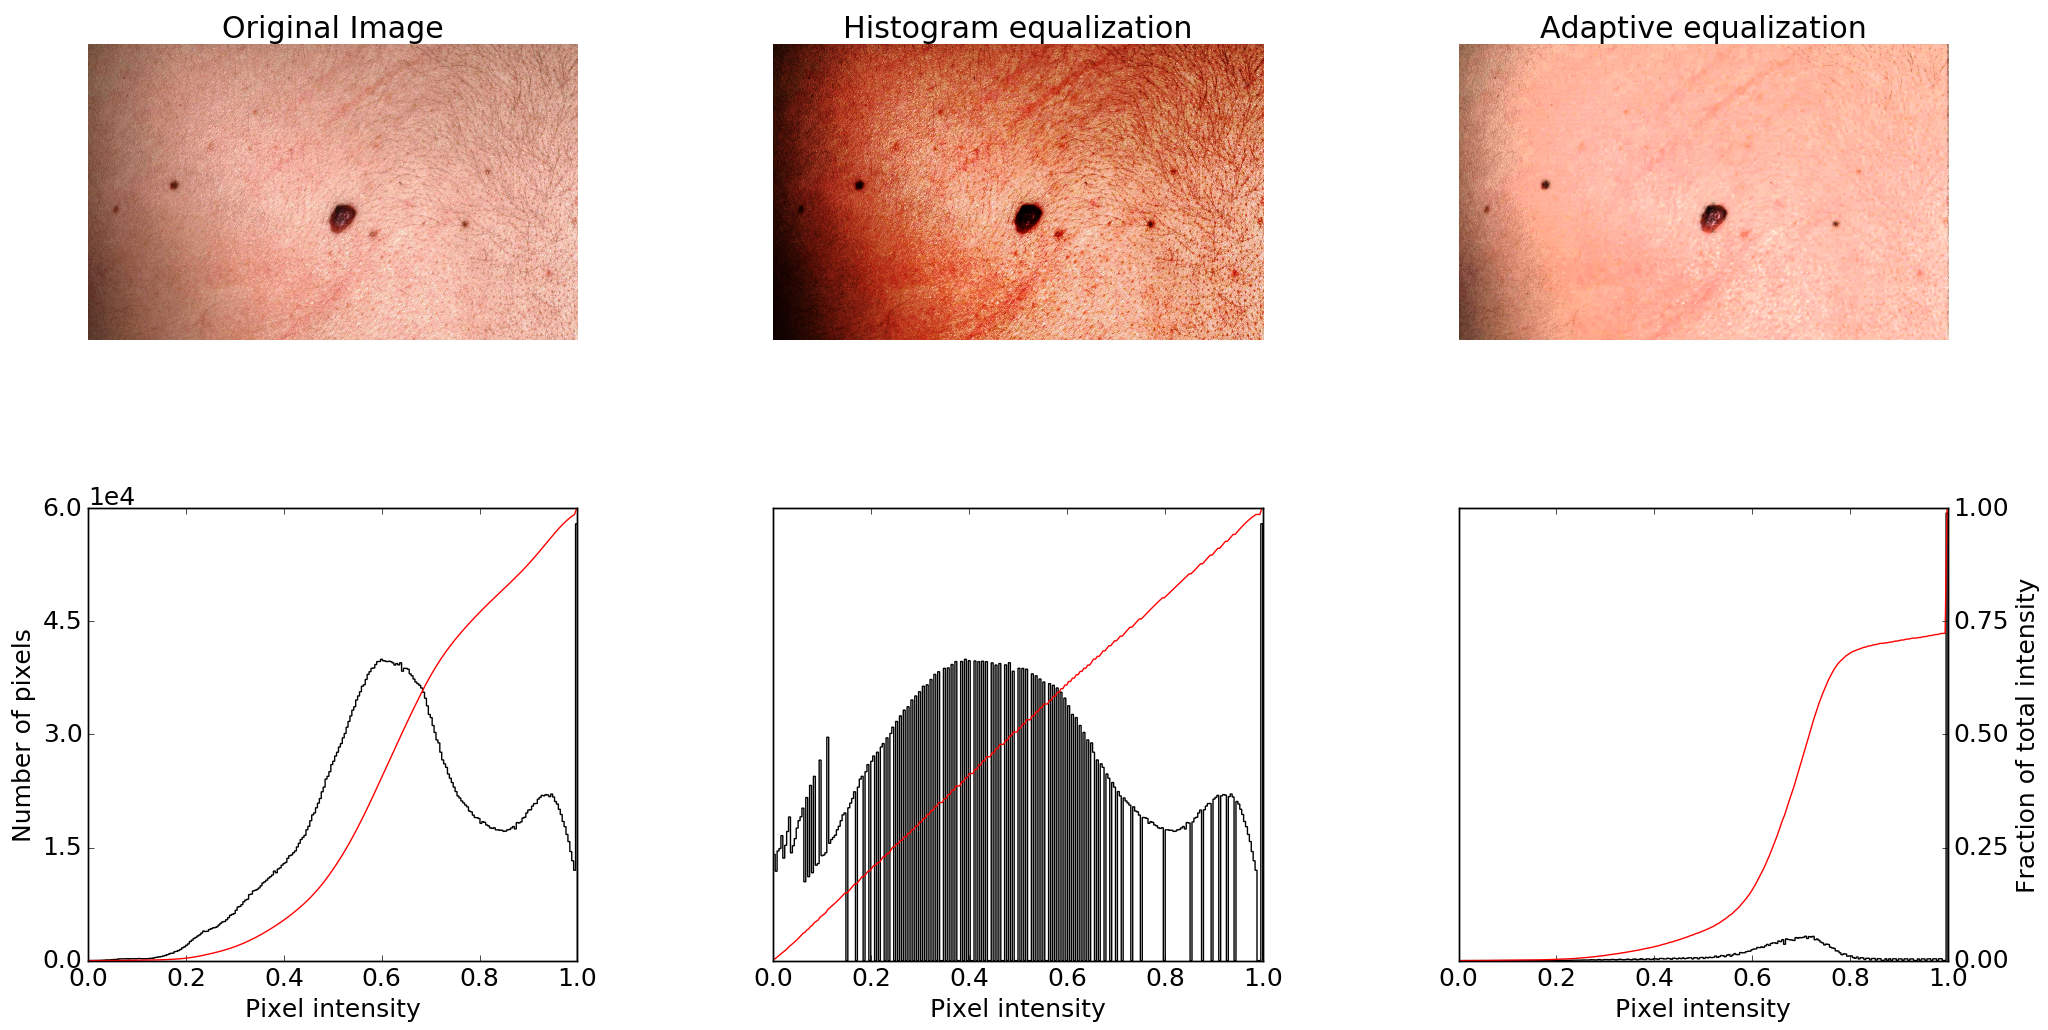
\includegraphics[width=\textwidth,keepaspectratio]{assets/image_processing/equalization/figure_01.png}
    \caption{Image Equalization Example A}
    \label{fig:eq_A}
\end{figure}
\begin{figure}[H]
    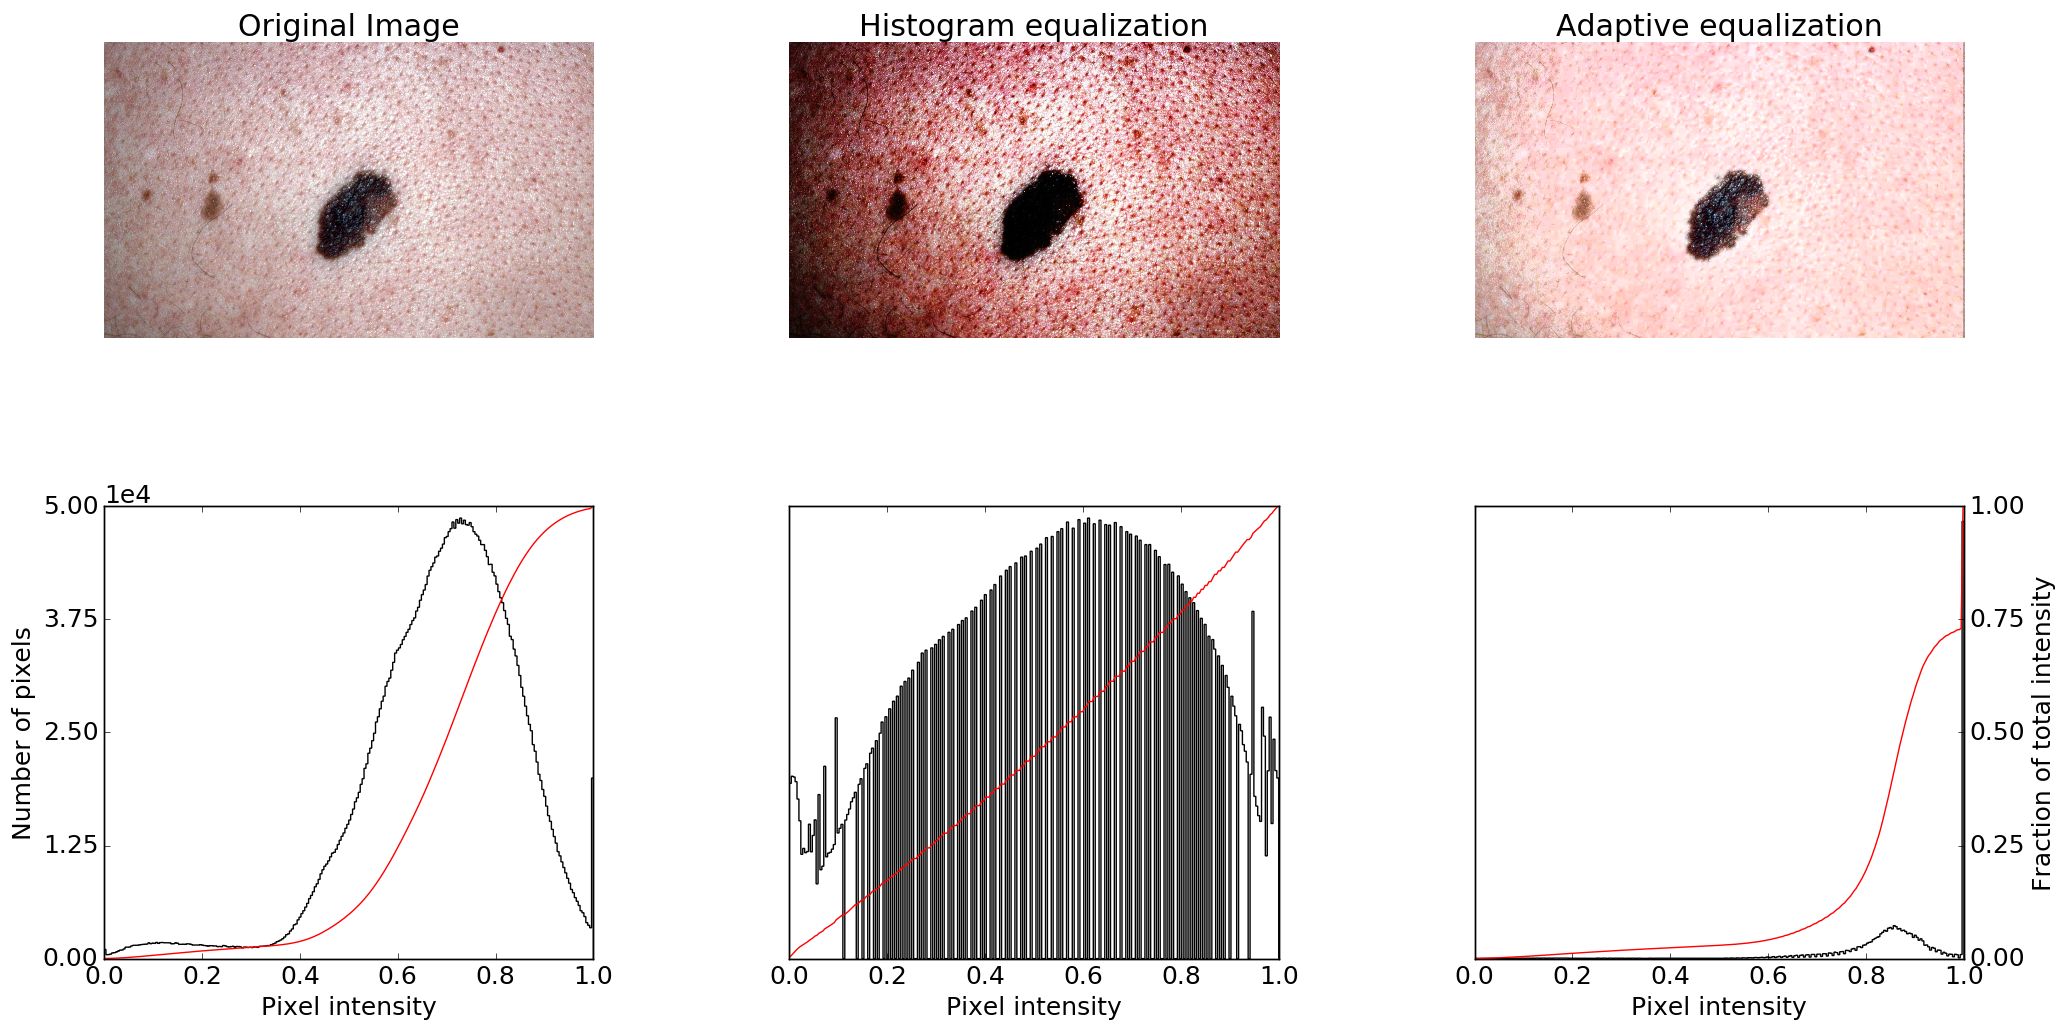
\includegraphics[width=\textwidth,keepaspectratio]{assets/image_processing/equalization/figure_02.png}
    \caption{Image Equalization Example B}
    \label{fig:eq_B}
\end{figure}
\begin{figure}[H]
    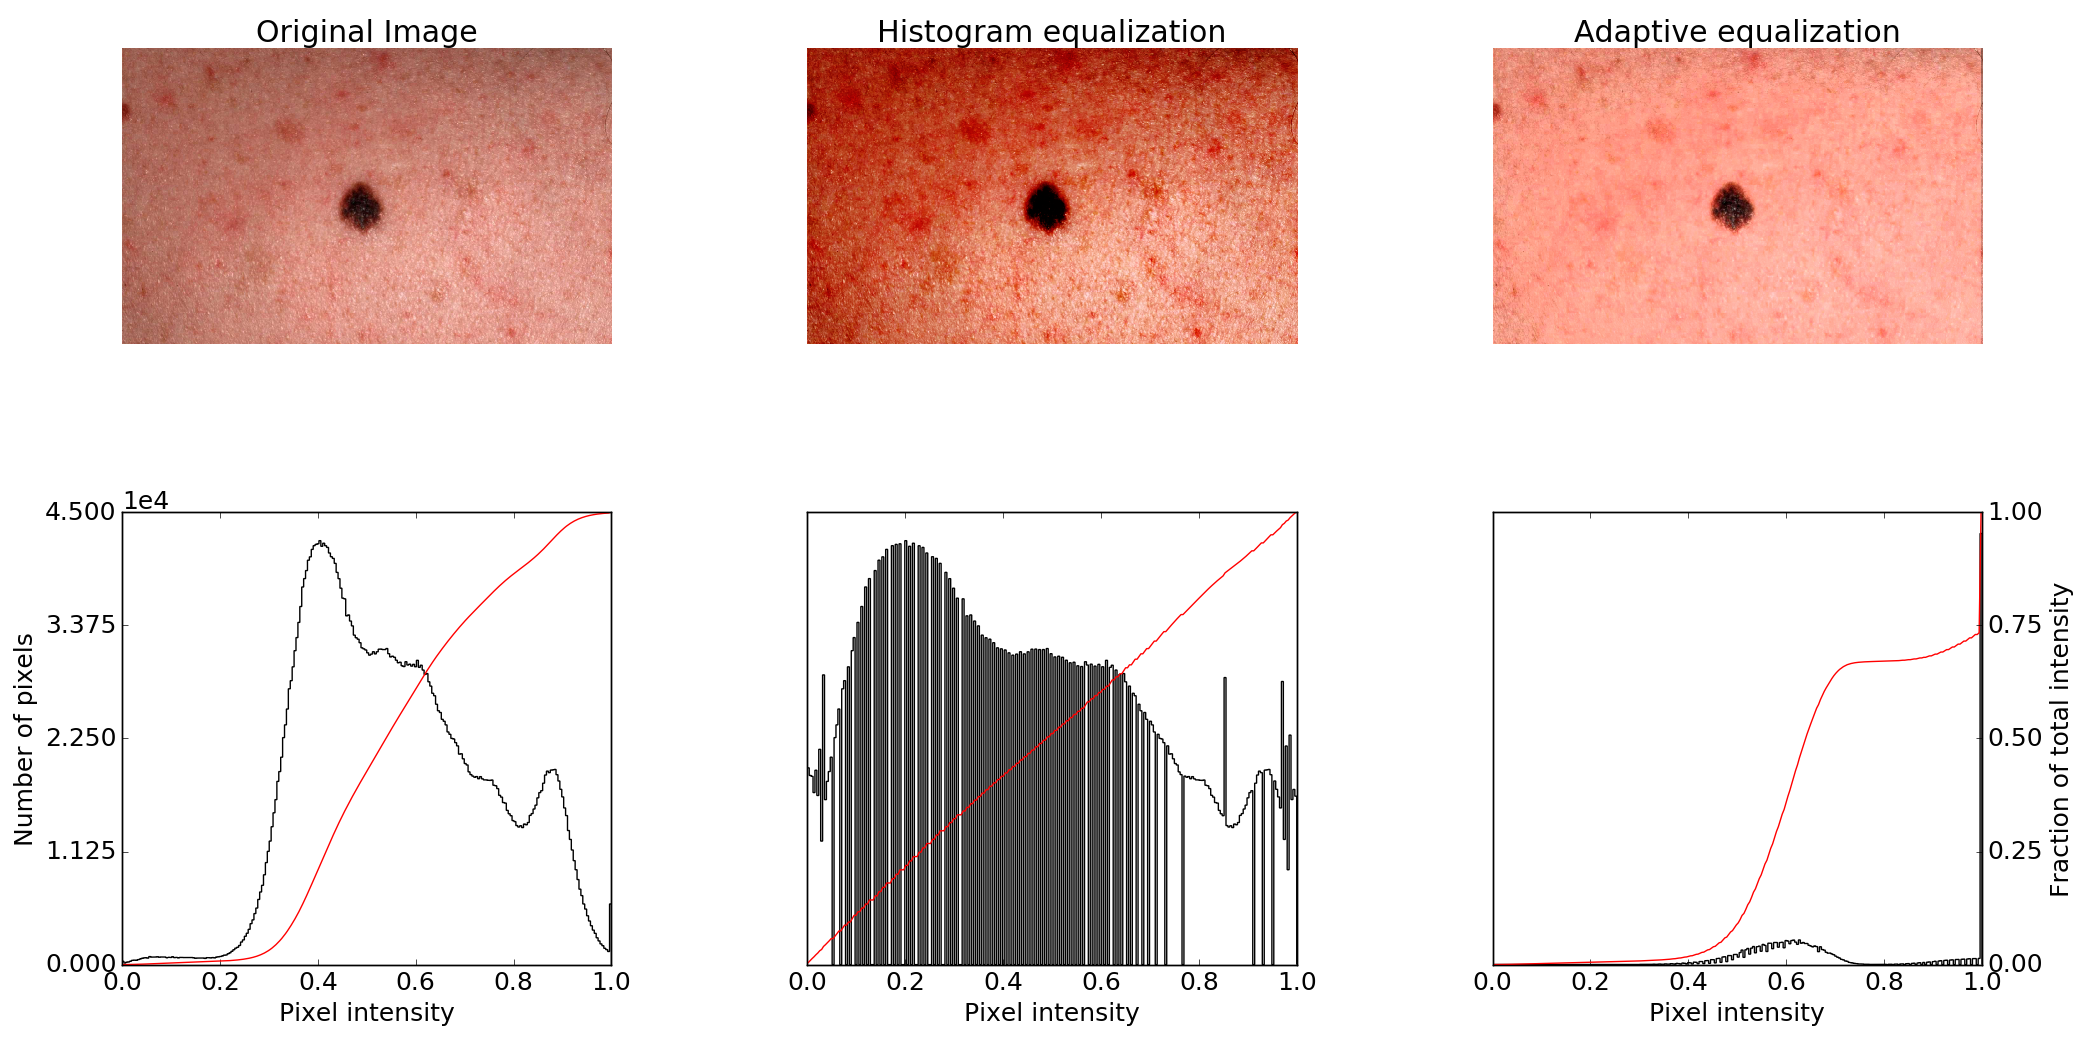
\includegraphics[width=\textwidth,keepaspectratio]{assets/image_processing/equalization/figure_03.png}
    \caption{Image Equalization Example C}
    \label{fig:eq_C}
\end{figure}

\subsection{Noise Reduction}

Noise in a captured image is inevitable, it will be introduced by the circuitry of the camera sensor or even from statistical quantum fluctuations of the photons known as “shot noise” \cite{image_noise}.  Noise in the image produces outlier pixels, pixels that do not represent the surface of the object in the image, and whose values diverge from neighbouring pixels.

Noise in the image will make it more difficult for the segmentation algorithms to achieve good accurate. Other challenges though might be reflectivity of the skin’s surface, the texture of the skin, or surrounding or intersecting the skin lesion.

Typical noise reduction techniques will analyse sections (often referred to as “windows” or “tiles”) or the image at a time and employ some sort of averaging function to the pixel values. Median or Gaussian filters are common noise reduction functions.

\subsubsection{Gaussian Blur}


\subsubsection{Median Filter}

The median filter will iterate through the pixels of an image, analysing each pixel and it's immediate neighbours. The value chosen for a pixels will be the median value of the area around the pixel. In a 2D context, if the neighbourhood around a pixel is [2,1,96] the pixel will receive the value 2. The median filter is easy to compute and has the quality that edges remain well preserved. This is therefore particularly useful as a preprocessing step before segmentation.

The following figures \ref{fig:med_A} to \ref{fig:med_C} are examples of median filtered images.

\begin{figure}[H]
    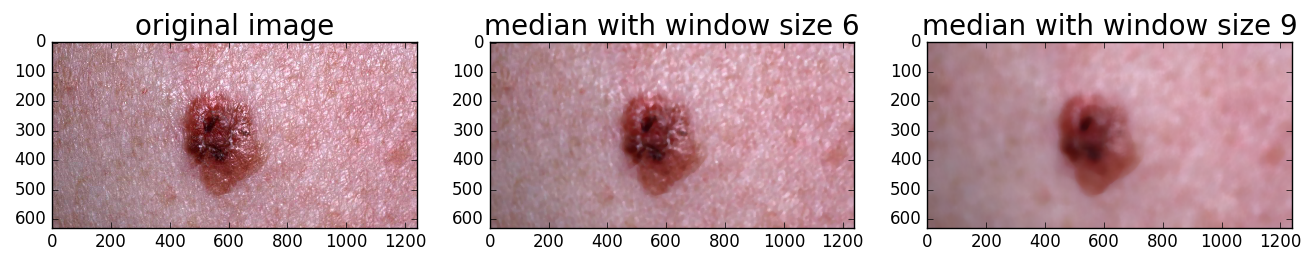
\includegraphics[width=\textwidth,keepaspectratio]{assets/image_processing/noise_reduction/figure_01.png}
    \caption{Median Filter Example A}
    \label{fig:med_A}
\end{figure}
\begin{figure}[H]
    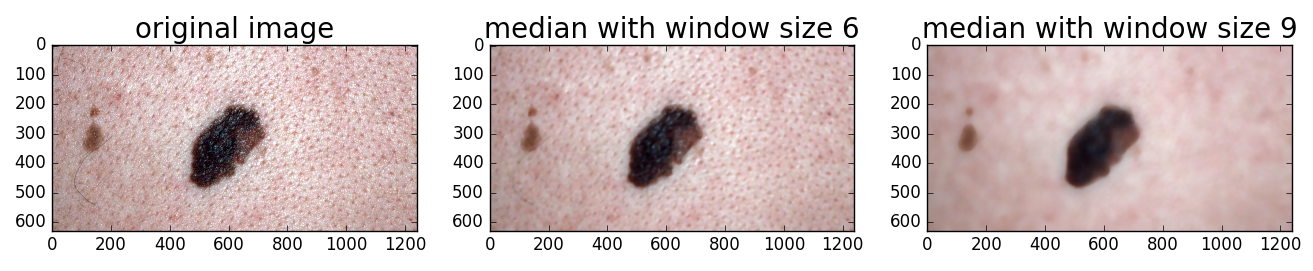
\includegraphics[width=\textwidth,keepaspectratio]{assets/image_processing/noise_reduction/figure_02.png}
    \caption{Median Filter Example B}
    \label{fig:med_B}
\end{figure}
\begin{figure}[H]
    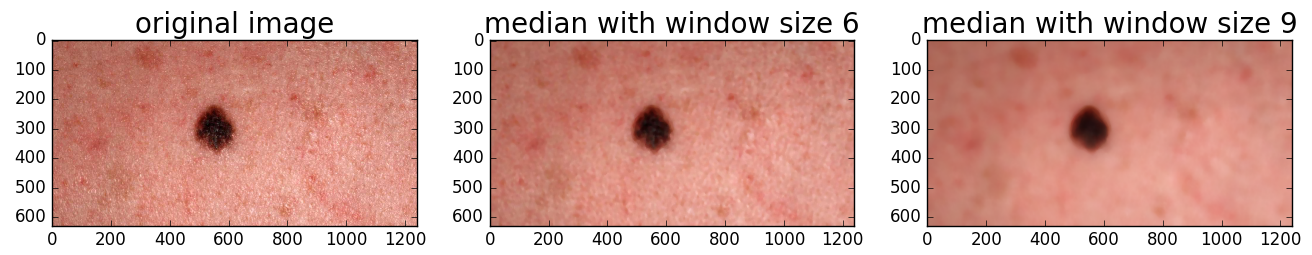
\includegraphics[width=\textwidth,keepaspectratio]{assets/image_processing/noise_reduction/figure_03.png}
    \caption{Median Filter Example C}
    \label{fig:med_B}
\end{figure}

The effect of the median window size is visible in the examples above. Larger window sizes are more effective at reducing noise and other disturbances. The edges of the lesion remain sharp, but the shape looses some detail, corners are rounded off. The size of the lesion in the image, and the image’s resolution are also important factors in the success of the median filter. If the lesion is too small compared to the image size, or the resolution of the image too low, then the shape will become more distorted. This will have a negative effect on the following segmentation steps.